\documentclass[a4paper,12pt]{report}
\usepackage{graphicx}
\usepackage[hidelinks]{hyperref}
\usepackage{geometry}
\usepackage{amsmath, amssymb, amsthm}
\usepackage{subcaption}
\usepackage{titlesec}
\usepackage{float}

\titleformat{\chapter}[display]
  {\normalfont\huge\bfseries}{\chaptertitlename\ \thechapter}{0pt}{\Huge}
\titlespacing*{\chapter}{0pt}{-40pt}{20pt}
\renewcommand{\bibname}{References}

\geometry{left=1.055118in, right=0.91in, top=1in, bottom=1in}

\graphicspath{{report image/}{images/}}

\begin{document}

% ==============================================================================
% COVER PAGE
% ==============================================================================
\begin{titlepage}
    \centering
    \vspace*{0.5cm}
    \Huge
    \textbf{MindCare}\\
    \large (Student Mental Health Support Application)\\
    \vfill
    \textit{\large A}\\
    \textbf{\textit{\Large Project Report}}\\
    \textit{submitted in partial fulfillment of the\\
    requirements for the award of the degree of}\\
    \vfill
    \textbf{\Large BACHELOR OF TECHNOLOGY}\\
    in\\
    \textbf{\Large COMPUTER SCIENCE \& ENGINEERING}\\
    (with specialization in \textbf{FULLSTACK\_AI})
    \vfill
    \textbf{by}\\
    \large
    \begin{tabular}{c c}
        \textbf{Name} & \textbf{Sap ID} \\ 
        Astha Gupta  & 500121750 \\
        Aastha Jaiswal & 500119719 \\
        Muskan Mittal & 500124380 \\
    \end{tabular}
    
    \vfill
    \textbf{\textit{under the guidance of}}\\
    \textbf{Mr. Vishal Kumar Lohan}
    \vfill
    
\includegraphics[width=0.4\textwidth]{UPES_logo.png}\\
    \vfill
    \textbf{School of Computer Science}\\
    \textbf{University of Petroleum \& Energy Studies}\\
    Bidholi, Via Prem Nagar, Dehradun, Uttarakhand\\
    \textbf{May -- 2026}
\end{titlepage}

% ==============================================================================
% CANDIDATE'S DECLARATION
% ==============================================================================
\pagebreak
\chapter*{\centering Candidate's Declaration}

\vspace{1cm}

I/We hereby certify that the project work entitled \textbf{``MindCare''} in partial fulfillment of the requirements for the award of the Degree of \textbf{BACHELOR OF TECHNOLOGY} in COMPUTER SCIENCE AND ENGINEERING with specialization in \textbf{FULLSTACK\_AI} and submitted to the \textbf{Department of Systemics}, School of Computer Science, University of Petroleum \& Energy Studies, Dehradun, is an authentic record of my/our work carried out during a period from \textbf{January, 2026} to \textbf{May, 2026} under the supervision of \textbf{Mr. Vishal Kumar Lohan, Assistant Professor}.

\vspace{0.5cm}

The matter presented in this project has not been submitted by me/us for the award of any other degree of this or any other University.

\vspace{1.5cm}

\begin{flushright}
    \textbf{(Astha Gupta \quad Sap id -- 500121750)} \\
    \textbf{(Aastha Jaiswal \quad Sap id -- 500119719)} \\
    \textbf{(Muskan Mittal \quad Sap id -- 500124380)}
\end{flushright}

\vspace{1.5cm}

This is to certify that the above statement made by the candidate is correct to the best of my knowledge.

\vspace{3cm}

\noindent
Date: 4/05/2026
\hfill
\begin{minipage}{5cm}
    \centering
    \textbf{\underline{( Mr. Vishal Kumar Lohan)}}\\
    Project Guide
\end{minipage}

\vfill
\hrule

% ==============================================================================
% ACKNOWLEDGEMENT
% ==============================================================================
\pagebreak
\chapter*{\centering Acknowledgement}

We wish to express our deep gratitude to our guide \textbf{Mr. Vishal Kumar Lohan}, for all advice, encouragement and constant support he has given us throughout our project work. This work would not have been possible without his support and valuable suggestions.\\

We sincerely thanks to our respected \textbf{Dr. Christalin Nelson S.}, Head Department of SOCS, for his great support in doing our project in \textbf{MindCare}. \\

We are also grateful to Dean SOCS UPES for giving us the necessary facilities to carry out our project work successfully. We also thanks to our Course Coordinator, (NAME) and our Activity Coordinator \textbf{Deepa Rani} for providing timely support and information during the completion of this project. \\ 

We would like to thank all our \textbf{friends} for their help and constructive criticism during our project work. Finally, we have no words to express our sincere gratitude to our \textbf{parents} who have shown us this world and for every support they have given us.

\vspace{3cm}

\begin{tabular}{l l l l}
    \textbf{Name} & \textbf{Astha Gupta} & \textbf{Aastha Jaiswal} & \textbf{Muskan Mittal} \\ 
    \textbf{Roll No.} & R2142230703 & R2142230323 & R2142231569 \\
\end{tabular}

\vfill
\hrule

% ==============================================================================
% ABSTRACT
% ==============================================================================
\chapter*{\centering Abstract}
\textbf{``MindCare''} -- The Holistic Mental Health and Wellness Companion is a project designed to address the increasing complexities of mental well-being, emotional regulation, proactive self-care, and personalized therapeutic support.

A mental wellness platform is a digital ecosystem that provides users with tools for emotional monitoring and psychological resilience without requiring immediate clinical intervention. These platforms are engineered to offer a safe, unstructured space for users to track their mental state and engage in wellness activities autonomously.

The goal of this project is to design and build a cross-platform mobile application that serves as a personal mental health assistant. The application must be able to track user moods in real-time, provide AI-driven conversational support, offer structured wellness exercises (such as breathing and grounding techniques), and facilitate a seamless connection between users and professional therapists.

The system is built using a React Native frontend and a Node.js/Express backend. It integrates \textbf{LangChain} and \textbf{Google GenAI} for its core intelligent component, an AI chatbot named ``Tink.'' Data persistence is managed through MongoDB, while Pinecone is utilized as a vector database to enable context-aware AI interactions, ensuring a highly personalized user experience.

The application is programmed to utilize advanced sentiment analysis for mood tracking and provides automated interventions based on user input. Therapeutic features like guided journaling, affirmations, and fitness coaching are integrated into a single interface. Once the system detects high stress levels, grounding techniques and crisis resources are prioritized to assist the user in regaining emotional stability.

One possible implementation of a digital wellness companion is to provide a preventative framework for mental health management. This function is useful in various sectors, including:
\begin{itemize}
    \item Personal Self-Care (Daily mood tracking and journaling)
    \item Clinical Support (Bridging the gap between patients and therapists)
    \item Corporate Wellness (Employee mental health monitoring)
    \item Crisis Management Systems
    \begin{itemize}
        \item Emergency Resource Access
        \item Immediate Grounding Interventions
        \item AI-based Emotional First Aid
    \end{itemize}
\end{itemize}


% ==============================================================================
% INDEX PAGES (TOC, LOF, LOT)
% ==============================================================================
\tableofcontents
\listoffigures
\listoftables



% ==============================================================================
% CHAPTER 1: INTRODUCTION
% ==============================================================================
\chapter{INTRODUCTION}
\section{Evolution of Digital Mental Healthcare}
\begin{itemize}
    \item \textbf{Background and Context}\\
    The global landscape of mental health has undergone a significant change in recent years, with increasing recognition of the importance of emotional well-being alongside physical health. Despite this, millions of individuals remain disadvantaged due to social stigma, high medical costs, and a shortage of mental health professionals. Digital health interventions have emerged as an important solution to bridge this gap.
    
    \item \textbf{The Role of AI in Wellness}\\
    Artificial Intelligence has transformed from a purely analytical tool to a helpful companion in the wellness sector. Modern applications now leverage natural language processing (NLP) to provide empathetic, real-time responses to users in crisis. \textbf{MindCare} uses these advancements to create a proactive rather than reactive mental health support system.
\end{itemize}

\section{Requirement Analysis}
\begin{itemize}
    \item \textbf{Problem Statement}\\
    The user could seamlessly shift between monitoring their daily wellness, journaling their thoughts, receiving conversational support, and connecting to a therapist---removing the need to use multiple applications for each purpose.
    
    \item \textbf{Targeted Users}\\
    The project primarily targets students, working professionals, and individuals looking for a private, low-barrier entry point into mental health management. By providing an autonomous tool, \textbf{MindCare} reduces the initial friction associated with seeking psychological help.
\end{itemize}

\section{Objectives}
\begin{itemize}
    \item \textbf{Main Objective}\\
    The \textbf{MindCare} project aims to use AI technology to build a mobile application that will integrate all aspects of mental, emotional, and therapeutic care.
    
    \item \textbf{Sub-Objectives}
    \begin{itemize}
        \item Develop a mood-check system to visualize users' emotional data over designated periods of time.
        \item Create ``Tink,'' an integrated, intelligent emotional support chatbot built on \textbf{LangChain} and \textbf{Google GenAI}.
        \item Integrate structured exercises, including guided therapeutic breathing, grounding activities, and gratitude journaling, to promote emotional wellness and balance.
        \item Provide a safe channel for interaction between clients and employed licensed practitioners.
    \end{itemize}
\end{itemize}

\section{Scope of the Project}
\begin{itemize}
    \item \textbf{Functional Boundaries}\\
    \textbf{MindCare} is designed to be a first-line support and well-being tracking tool. Although it provides AI-powered interactions and resources, it is intended to complement, not replace, clinical psychiatric diagnosis. The project focuses on data-driven insights and immediate coping mechanisms to improve the quality of daily life of the user.
\end{itemize}


% ==============================================================================
% CHAPTER 2: SYSTEM ANALYSIS
% ==============================================================================
\chapter{SYSTEM ANALYSIS}
\section{Existing System}
Traditional approaches to mental health management rely primarily on face-to-face therapy sessions and manual self-tracking methods. Currently, many users use simple note-taking apps or physical journals to record their feelings. However, these existing methods have several limitations:
\begin{itemize}
    \item \textbf{Lack of immediate response:} Standard magazines may not provide feedback or emotional support during a crisis.
    \item \textbf{High barrier to entry:} Occupational therapy is often expensive and requires scheduling, making it inaccessible for immediate, daily needs.
    \item \textbf{Data fragmentation:} Users often have their wellness data (fitness, mood, thoughts) spread across multiple unrelated platforms.
    \item \textbf{Stigma and confidentiality:} Many individuals avoid seeking help due to the perceived stigma of attending a clinic.
\end{itemize}

\begin{itemize}
    \item \textbf{Technical Framework}\\
    React Native offers cross-platform access, Node.js provides a flexible backend, and \textbf{Pinecone Vector Database} ensures personalized, context-based responses from the AI, grounded in therapeutic best practices. So, this project employs a contemporary technology stack, project describing its component functionalities.
\end{itemize}

\section{Motivations}
The main goal of \textbf{MindCare} is to facilitate access to mental health support through technology. The development of Large Language Models (LLMs) and mobile computing paves the way for a sentimental and personalized companion that can be present 24/7. What \textbf{MindCare} aims for is to create a ``safe space'' that gives data-informed insight and AI-driven therapy that works to inspire and encourage the user to be more engaged with their mental health.

\section{Proposed System}
The proposed system, \textbf{MindCare}, is an integrated mental wellness ecosystem built on a mobile-first architecture. It integrates proactive mood monitoring with responsive AI conversational support. Unlike the existing system, \textbf{MindCare} provides:
\begin{itemize}
    \item \textbf{24/7 AI Interaction:} An intelligent chatbot (Tink) that provides immediate emotional support.
    \item \textbf{Holistic data integration:} A single platform for journaling, mood tracking, and fitness monitoring.
    \item \textbf{Contextual Intelligence:} Uses vector databases to ``remember'' user history and provide more relevant support over time.
    \item \textbf{Professional Connectivity:} A secure bridge for users to transition from self-care to professional therapy when needed.
\end{itemize}

\section{Modules}
\begin{itemize}
    \item \textbf{AI Conversational Engine (Tink)}\\
    This is the main intelligence module of the app. It uses \textbf{LangChain} and \textbf{Google GenAI} to process user messages and provide empathetic responses. This module also interacts with the Pinecone vector database to maintain long-term context and ensure continuity of interaction.
    
    \item \textbf{Emotional Analytics \& Mood Tracker}\\
    This module handles the collection and visualization of the user's emotional state. It allows users to log their mood daily and generates graphical insights (trends, triggers) to help users understand their psychological patterns over weeks or months.
    
    \item \textbf{Therapeutic Toolkit (Activities)}\\
    This module includes various non-interactive wellness tools:
    \begin{itemize}
        \item \textbf{Guided Breathing:} Interactive animations to help users control their heart rate.
        \item \textbf{Grounding exercise:} A technique for bringing attention back to the present moment during anxiety.
        \item \textbf{Gratitude Journal:} A dedicated space for positive reflection.
    \end{itemize}
    
    \item \textbf{Therapist-Patient Interface}\\
    A special module designed for health care professionals. It allows physicians to view authorization data from their patients, manage appointments, and provide direct feedback through a dedicated dashboard.
    
    \item \textbf{User Management \& Security}\\
    This module handles secure authentication using \textbf{JWT (JSON Web Token)} and \textbf{bcryptjs} for password hashing. This ensures that sensitive mental health data is encrypted and only accessible to authorized users.
\end{itemize}


% ==============================================================================
% CHAPTER 3: DESIGN
% ==============================================================================
\chapter{DESIGN}
\section{System Architecture \& Modeling}
\subsection{Architecture and Behavioral Logic}
MindCare's design is centered around a responsive behavior model. Unlike traditional static apps, \textbf{MindCare} behaves like a living assistant. It uses a client-server architecture where the mobile frontend handles the user experience, while the backend manages ``cognitive'' tasks such as sentiment analysis and episodic memory.

\section{Use Case Model for Requirement Analysis}
\begin{figure}[H]
    \centering
    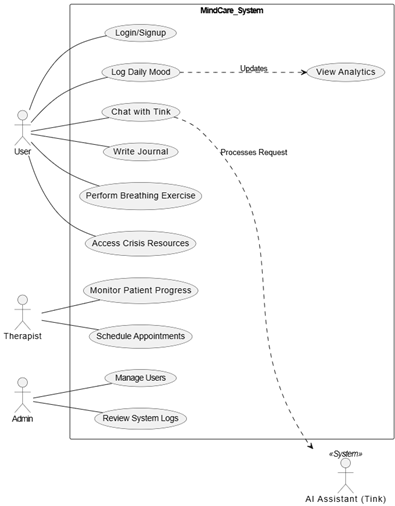
\includegraphics[width=0.65\textwidth]{use-case-diagram.png}
    \caption{Fig. 3.1: Use Cases Model for the System}
    \label{fig:use_case}
\end{figure}
The use case diagram identifies the main functionality of the system. The primary actor is the user, who triggers events such as logging a mood or starting a chat. The AI assistant (Tink) serves as a secondary system actor that processes these inputs to provide therapeutic grounding. The therapist actor interacts with the system to review longitudinal data, ensuring a hybrid care approach.

\section{The Design Model}
\begin{figure}[H]
    \centering
    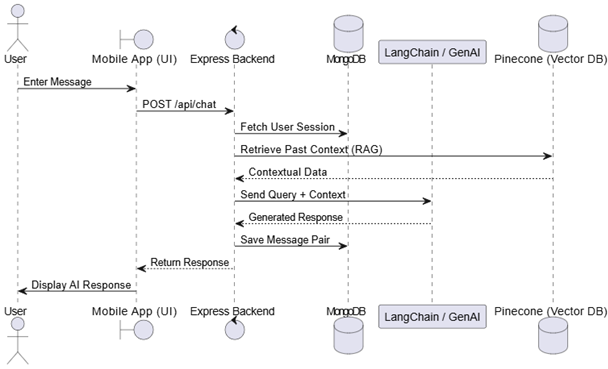
\includegraphics[width=0.65\textwidth]{sequence-diagram.png}
    \caption{Fig. 3.2: Sequence}
    \label{fig:sequence}
\end{figure}
The design model is illustrated through a sequence diagram. It captures time-ordered interactions between system components. When a user sends a message, the system executes a ``Retrieval Augmented Generation'' (RAG) cycle. This involves deriving previous emotional context from the Pinecone Vector database before generating a response, ensuring that the interaction feels personal and sustained.

\section{Object and Class Design}
\begin{figure}[H]
    \centering
    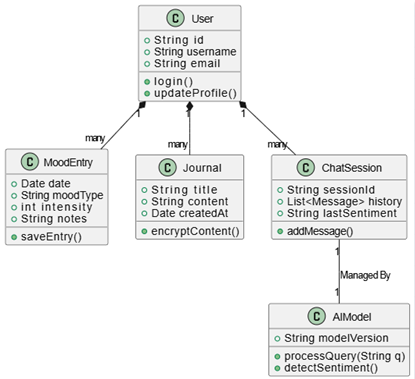
\includegraphics[width=0.7\textwidth]{class-diagram.png}
    \caption{Class Diagram}
    \label{fig:class_diagram}
\end{figure}
The class design represents the static structure of the \textbf{MindCare} database. The User class is the central entity, which has a one-to-many relationship with Moodlogs and Journals. This encapsulation ensures that user data is logically organized, allowing efficient queries when generating progress reports or sentiment trends.

\section{State Transition}
\begin{figure}[H]
    \centering
    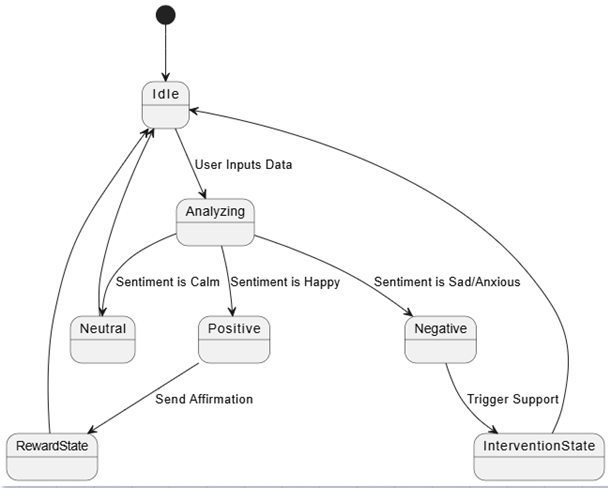
\includegraphics[width=0.7\textwidth]{state-transition-mood-detection-behaviour.png}
    \caption{Fig. 3.4: Mood Detection Behavior}
    \label{fig:state_mood}
\end{figure}

\begin{figure}[H]
    \centering
    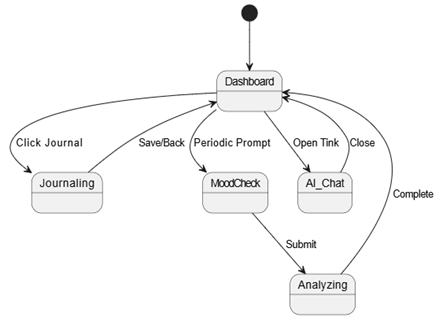
\includegraphics[width=0.7\textwidth]{state-transition-app-feature-navigation.png}
    \caption{Fig. 3.5: State Transition: App Feature Navigation}
    \label{fig:state_nav}
\end{figure}


\begin{figure}[H]
    \centering
    \includegraphics[height=0.35\textheight, keepaspectratio]{state_crisis.png}
    \caption{Fig. 3.6: State Transition: Crisis Interruption (Obstacle Avoidance)}
    \label{fig:state_crisis}
\end{figure}

\begin{figure}[H]
    \centering
    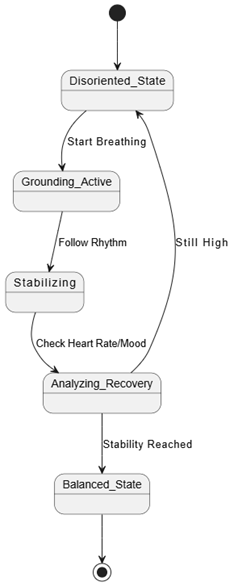
\includegraphics[height=0.35\textheight, keepaspectratio]{state-transition-emotional-recovery.png}
    \caption{Fig. 3.7: State Transition: Emotional Recovery (Restoring Path)}
    \label{fig:state_recovery}
\end{figure}



System logic is controlled by several state machines:
\begin{itemize}
    \item \textbf{Mood detection (3.4):} Transition between 'neutral', 'positive' and 'negative' based on NLP analysis.
    \item \textbf{Finding Path (3.5):} Manages the user's journey through various app modules (for example, from Dashboard to Therapy).
    \item \textbf{Barrier resolution (3.6):} This represents ``crisis handling''. If high voltage is detected, the app interrupts the normal flow to provide immediate grounding resources.
    \item \textbf{Restoration Path (3.7):} This represents the ``recovery flow'', which guides the user from the crisis state back to a balanced emotional baseline.
\end{itemize}

\section{Activity Diagram}
\begin{figure}[H]
    \centering
    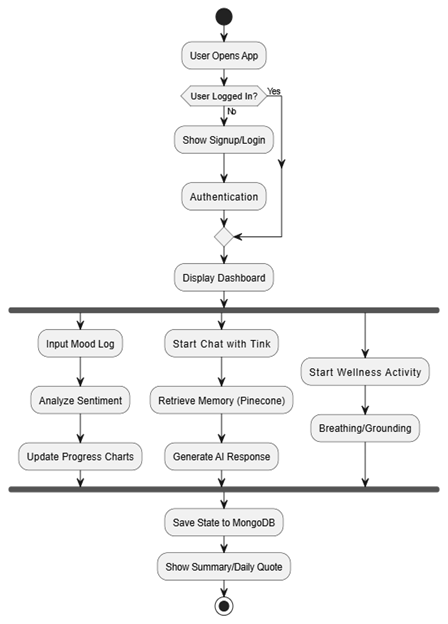
\includegraphics[width=0.65\textwidth]{activity-diagram.png}
    \caption{Fig. 3.8: Activity Diagram for the System}
    \label{fig:activity}
\end{figure}
Activity diagrams provide the high-level workflow of a system's operational logic. It starts with authentication checks, followed by the main dashboard loop. The diagram highlights the parallel processing of mood logging and AI interactions, showing how the system concludes each session by saving the data in the MongoDB cloud and providing daily motivational results to the user.


% ==============================================================================
% CHAPTER 4: MINDCARE
% ==============================================================================
\chapter{MINDCARE}
\section{MindCare Application Overview}
\textbf{MindCare} is a holistic wellness platform designed to bridge the gap between traditional medicine and self-care. It provides a centralized hub for mood tracking, AI-powered conversations, and guided therapeutic exercises.

\begin{figure}[H]
    \centering
    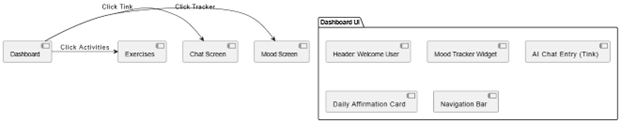
\includegraphics[width=0.65\textwidth]{app-logo-dashboard.png}
    \caption{Fig. 4.1: MindCare App Logo and Dashboard}
    \label{fig:dashboard}
\end{figure}

\section{LangChain \& GenAI – The System’s Brain}
The ``brain'' of the \textbf{MindCare} system is an orchestration layer powered by \textbf{LangChain}. This layer connects the user interface to the larger language model, ensuring that interactions are structured and therapeutically based.

\subsection{Technical Specifications}
The system leverages the \textbf{Gemini API} for its core reasoning capabilities. The integration allows for high-speed Natural Language Processing and sentiment detection.

\subsection{Knowledge Organization – Vector Database (Pinecone)}
To ensure the AI has ``long-term memory,'' \textbf{MindCare} uses a vector database. This organizes user data into mathematical vectors, allowing the AI to retrieve relevant past interactions to provide contextually accurate support.

\begin{figure}[H]
    \centering
    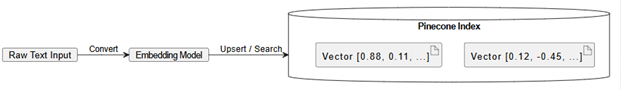
\includegraphics[width=0.95\textwidth]{pinecone-vector-storage-structure.png}
    \caption{Fig. 4.2: Pinecone Vector Storage Structure}
    \label{fig:pinecone}
\end{figure}

\section{Developing the MindCare Environment}
The development of \textbf{MindCare} utilizes a \textbf{Node.js} backend and a \textbf{React Native} frontend. The backend manages secure API routing and database connections.

\begin{figure}[H]
    \centering
    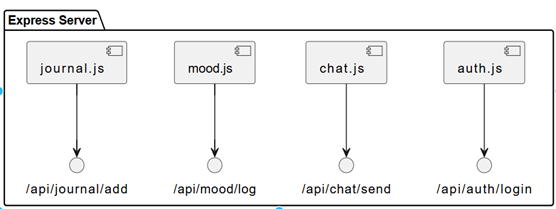
\includegraphics[width=0.95\textwidth]{nodejs-backend-api-routes.png}
    \caption{Fig. 4.3: Node.js Backend \& API Routes}
    \label{fig:backend_routes}
\end{figure}

\begin{figure}[H]
    \centering
    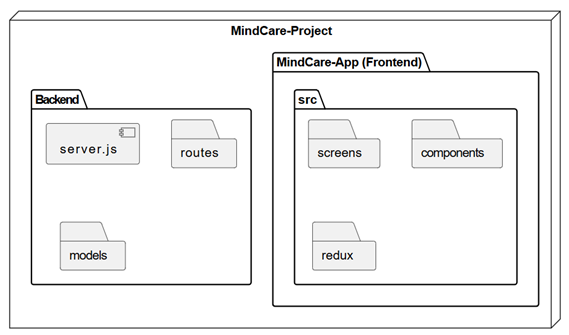
\includegraphics[width=0.95\textwidth]{react-native-codebase-structure.png}
    \caption{Fig. 4.4: React Native Codebase Structure}
    \label{fig:react_native}
\end{figure}

\begin{table}[ht!]
    \centering
    \begin{tabular}{|l|l|l|}
        \hline
        \textbf{Endpoint} & \textbf{Method} & \textbf{Description} \\ \hline
        /api/auth/login & POST & User Authentication \\ \hline
        /api/mood/log & POST & Log Daily Mood \\ \hline
        /api/chat/send & POST & Send Message to Tink \\ \hline
        /api/journal/add & POST & Save Journal Entry \\ \hline
    \end{tabular}
    \caption{MindCare Core API Endpoints and HTTP Methods}
    \label{tab:api_endpoints}
\end{table}

\subsection{Environment Setup \& Quick Start}
Initializing the project requires running the Metro bundler to compile the JavaScript code for mobile deployment.

\begin{figure}[H]
    \centering
    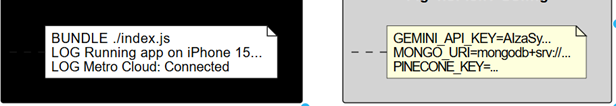
\includegraphics[width=0.95\textwidth]{metro-bundler-console-output.png}
    \caption{Fig. 4.5: Metro Bundler Console Output}
    \label{fig:metro}
\end{figure}

Before running the app, environment variables must be configured to securely store the API keys for \textbf{LangChain} and \textbf{MongoDB}. The app is then deployed on an emulator or physical device for testing. During development, the debug terminal is used to monitor the live data exchange between the app and the AI server.

\section{The Interaction Layer – React Native UI Components}
The user interface is built using modular \textbf{React Native} components. These components ensure a smooth transition between screens, such as moving from the Dashboard to a Breathing Exercise.

\section{The ``Sensors'' – Sentiment Analysis Engine}
\textbf{MindCare's} primary way of ``sensing'' the user's state is through its sentiment analysis logic. This logic categorizes text into emotional zones to determine the type of support needed.

\begin{figure}[H]
    \centering
    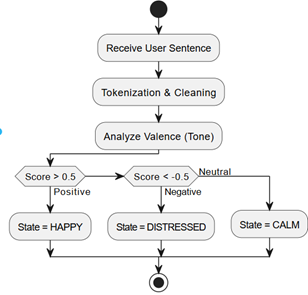
\includegraphics[width=0.95\textwidth]{sentiment-detection-logic-using-nlp.png}
    \caption{Fig. 4.6: Sentiment Detection Logic using NLP}
    \label{fig:sentiment_logic}
\end{figure}

\begin{figure}[H]
    \centering
    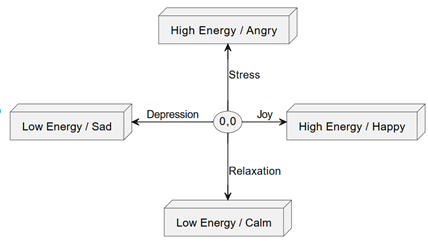
\includegraphics[width=0.7\textwidth]{mood-intensity-mapping-graph.png}
    \caption{Fig. 4.7: Mood Intensity Mapping Graph}
    \label{fig:mood_mapping}
\end{figure}

\section{Real-time Monitoring – Threshold Detection}
The system constantly monitors emotional ``thresholds.'' If the sentiment analysis detects a score that indicates high distress, the system triggers an immediate safety intervention.

\begin{figure}[H]
    \centering
    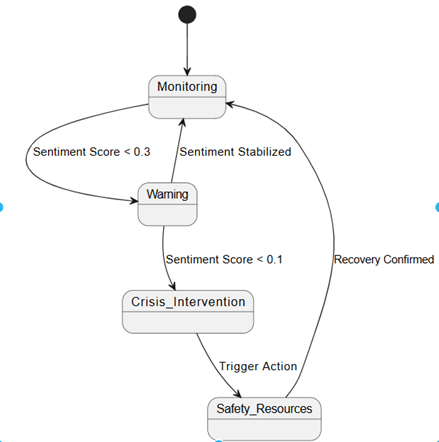
\includegraphics[width=0.7\textwidth]{real-time-stress-level-threshold-monitor.png}
    \caption{Fig. 4.8: Real-time Stress Level Threshold Monitor}
    \label{fig:threshold}
\end{figure}


% ==============================================================================
% CHAPTER 5: IMPLEMENTATION
% ==============================================================================
\chapter{Implementation}
\section{Emotional State Mapping using Sentiment Scoring}
In \textbf{MindCare}, ``Path Tracing'' refers to monitoring a user's emotional baseline over time. Instead of Cartesian X and Y coordinates, we use Sentiment Valence (positive/negative) and Arousal/Intensity as our two-dimensional coordinate system to map the user's mental state.

\begin{figure}[H]
    \centering
    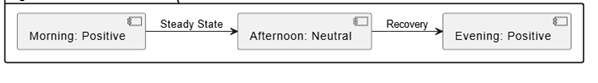
\includegraphics[width=0.8\textwidth]{emotional-journey-graph.png}
    \caption{Emotional Journey Graph (Stable baseline)}
    \label{fig:journey_stable}
\end{figure}

When a user faces stress or anxiety, these act as ``obstacles'' in their emotional path. The system must detect these peaks and provide a ``restoration path'' to bring the user back to their psychological baseline.

\begin{figure}[H]
    \centering
    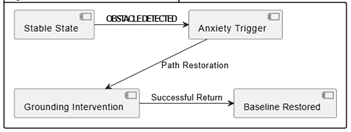
\includegraphics[width=0.8\textwidth]{emotional-journey-graph-with-crisis.png}
    \caption{Emotional Journey Graph (With crisis ``obstacles'')}
    \label{fig:journey_crisis}
\end{figure}

\section{Operational Scenarios}
The implementation of \textbf{MindCare} is tested based on three primary scenarios:
\begin{enumerate}
    \item \textbf{Daily Maintenance:} Where the user is stable and requires regular tracking.
    \item \textbf{Crisis intervention:} Where an acute decline in mood (a disturbance) is detected.
    \item \textbf{Long-term recovery:} Where the system scans past patterns to prevent future triggers.
\end{enumerate}

\section{Behavioral Algorithms}
\textbf{Algorithm 1: Sentiment-Based Support Selection}\\
This algorithm functions similarly to ``Coordinate Based Seeking.'' It takes the current sentiment score (the ``coordinate'') and calculates the direct path to the most appropriate supportive response or grounding exercise.

\begin{figure}[H]
    \centering
    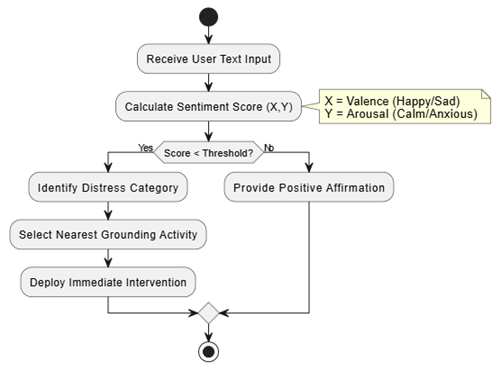
\includegraphics[width=0.6\textwidth]{direct-sentiment-scenario1.png}
    \caption{Scenario-1: Direct Sentiment-Based Support Flow}
    \label{fig:algo_support}
\end{figure}

\textbf{Algorithm 2: Pattern-Based Activity Recommendation}\\
Similar to ``Lookup Based Seeking,'' this algorithm does not just look at the current score but looks up the user's history in the database. If the user previously found a ``Breathing Exercise'' helpful during a similar mood, the system prioritizes that recommendation.

\begin{figure}[H]
    \centering
    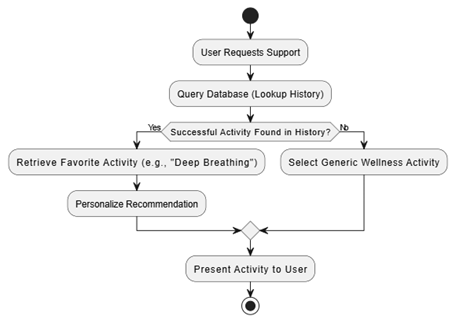
\includegraphics[width=0.6\textwidth]{pattern-based-scenerio2.png}
    \caption{Scenario-2: Pattern-Based Exercise Recommendation}
    \label{fig:algo_pattern}
\end{figure}

\textbf{Algorithm 3: Holistic Wellness Scanning}\\
Inspired by ``Serpentine Scanning,'' this algorithm performs a comprehensive scan of all user inputs (Journals, Fitness logs, and Chat history). It weaves through these different data points to find ``hidden'' trends that a single mood log might miss, ensuring a holistic view of the user's well-being.

\begin{figure}[H]
    \centering
    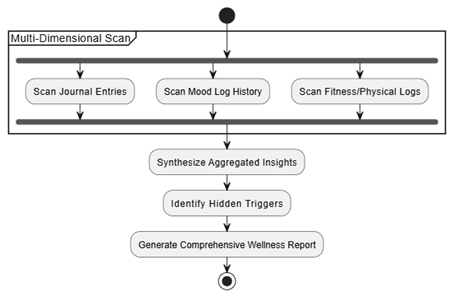
\includegraphics[width=0.8\textwidth]{holistic-scanning-scenerio3.png}
    \caption{Scenario-3: Holistic Scanning of User Metadata}
    \label{fig:algo_holistic}
\end{figure}

% ==============================================================================
% CHAPTER 6: OUTPUT SCREENS
% ==============================================================================
\chapter{Output Screens}
This section showcases the final user interface of the \textbf{MindCare} application, divided into the various portals used by different stakeholders.

\section{Login and Signup}
\begin{figure}[H]
    \centering
    \begin{subfigure}[b]{0.45\textwidth}
        \centering
        
\includegraphics[width=\textwidth, height=0.25\textheight, keepaspectratio]{report image/report image/1.jpeg}
        \caption{Screen 1}
    \end{subfigure}
    \hfill
    \begin{subfigure}[b]{0.45\textwidth}
        \centering
        
\includegraphics[width=\textwidth, height=0.25\textheight, keepaspectratio]{report image/report image/2.jpeg}
        \caption{Screen 2}
    \end{subfigure}
    \caption{Authentication Screens}
\end{figure}

\section{Therapist Portal}
\begin{figure}[H]
    \centering
    \begin{subfigure}[b]{0.45\textwidth}
        \centering
        
\includegraphics[width=\textwidth, height=0.25\textheight, keepaspectratio]{report image/report image/3.jpeg}
        \caption{Screen 3}
    \end{subfigure}
    \hfill
    \begin{subfigure}[b]{0.45\textwidth}
        \centering
        
\includegraphics[width=\textwidth, height=0.25\textheight, keepaspectratio]{report image/report image/4.jpeg}
        \caption{Screen 4}
    \end{subfigure}
    \caption{Therapist Portal Screens}
\end{figure}

\section{Patient Portal}
\begin{figure}[H]
    \centering
    \begin{subfigure}[b]{0.3\textwidth}
        \centering
        
\includegraphics[width=\textwidth, height=0.35\textheight, keepaspectratio]{report image/report image/5.jpeg}
        \caption{Screen 5}
    \end{subfigure}
    \hfill
    \begin{subfigure}[b]{0.3\textwidth}
        \centering
        
\includegraphics[width=\textwidth, height=0.35\textheight, keepaspectratio]{report image/report image/6.jpeg}
        \caption{Screen 6}
    \end{subfigure}
    \hfill
    \begin{subfigure}[b]{0.3\textwidth}
        \centering
        
\includegraphics[width=\textwidth, height=0.35\textheight, keepaspectratio]{report image/report image/7.jpeg}
        \caption{Screen 7}
    \end{subfigure}
    \vspace{0.5cm}

    \begin{subfigure}[b]{0.3\textwidth}
        \centering
        
\includegraphics[width=\textwidth, height=0.35\textheight, keepaspectratio]{report image/report image/8.jpeg}
        \caption{Screen 8}
    \end{subfigure}
    \hfill
    \begin{subfigure}[b]{0.3\textwidth}
        \centering
        
\includegraphics[width=\textwidth, height=0.35\textheight, keepaspectratio]{report image/report image/9.jpeg}
        \caption{Screen 9}
    \end{subfigure}
    \hfill
    \begin{subfigure}[b]{0.3\textwidth}
        \centering
        
\includegraphics[width=\textwidth, height=0.35\textheight, keepaspectratio]{report image/report image/10.jpeg}
        \caption{Screen 10}
    \end{subfigure}
    \caption{Patient Portal Screens (Part 1)}
\end{figure}

\begin{figure}[H]
    \centering
    \begin{subfigure}[b]{0.3\textwidth}
        \centering
        
\includegraphics[width=\textwidth, height=0.35\textheight, keepaspectratio]{report image/report image/11.jpeg}
        \caption{Screen 11}
    \end{subfigure}
    \hfill
    \begin{subfigure}[b]{0.3\textwidth}
        \centering
        
\includegraphics[width=\textwidth, height=0.35\textheight, keepaspectratio]{report image/report image/12.jpeg}
        \caption{Screen 12}
    \end{subfigure}
    \hfill
    \begin{subfigure}[b]{0.3\textwidth}
        \centering
        
\includegraphics[width=\textwidth, height=0.35\textheight, keepaspectratio]{report image/report image/13.jpeg}
        \caption{Screen 13}
    \end{subfigure}
    \vspace{0.5cm}

    \begin{subfigure}[b]{0.3\textwidth}
        \centering
        
\includegraphics[width=\textwidth, height=0.35\textheight, keepaspectratio]{report image/report image/14.jpeg}
        \caption{Screen 14}
    \end{subfigure}
    \hfill
    \begin{subfigure}[b]{0.3\textwidth}
        \centering
        
\includegraphics[width=\textwidth, height=0.35\textheight, keepaspectratio]{report image/report image/15.jpeg}
        \caption{Screen 15}
    \end{subfigure}
    \caption{Patient Portal Screens (Part 2)}
\end{figure}

\section{Admin Portal}
\begin{figure}[H]
    \centering
    \begin{subfigure}[b]{0.3\textwidth}
        \centering
        
\includegraphics[width=\textwidth, height=0.35\textheight, keepaspectratio]{report image/report image/16.jpeg}
        \caption{Screen 16}
    \end{subfigure}
    \hfill
    \begin{subfigure}[b]{0.3\textwidth}
        \centering
        
\includegraphics[width=\textwidth, height=0.35\textheight, keepaspectratio]{report image/report image/17.jpeg}
        \caption{Screen 17}
    \end{subfigure}
    \hfill
    \begin{subfigure}[b]{0.3\textwidth}
        \centering
        
\includegraphics[width=\textwidth, height=0.35\textheight, keepaspectratio]{report image/report image/18.jpeg}
        \caption{Screen 18}
    \end{subfigure}
    \vspace{0.5cm}

    \begin{subfigure}[b]{0.3\textwidth}
        \centering
        
\includegraphics[width=\textwidth, height=0.35\textheight, keepaspectratio]{report image/report image/19.jpeg}
        \caption{Screen 19}
    \end{subfigure}
    \hfill
    \begin{subfigure}[b]{0.3\textwidth}
        \centering
        
\includegraphics[width=\textwidth, height=0.35\textheight, keepaspectratio]{report image/report image/20.jpeg}
        \caption{Screen 20}
    \end{subfigure}
    \hfill
    \begin{subfigure}[b]{0.3\textwidth}
        \centering
        
\includegraphics[width=\textwidth, height=0.35\textheight, keepaspectratio]{report image/report image/21.jpeg}
        \caption{Screen 21}
    \end{subfigure}
    \caption{Admin Portal Screens (Part 1)}
\end{figure}

\begin{figure}[H]
    \centering
    \begin{subfigure}[b]{0.3\textwidth}
        \centering
        
\includegraphics[width=\textwidth, height=0.35\textheight, keepaspectratio]{report image/report image/22.jpeg}
        \caption{Screen 22}
    \end{subfigure}
    \caption{Admin Portal Screens (Part 2)}
\end{figure}

% ==============================================================================
% CHAPTER 7: LIMITATIONS AND FUTURE ENHANCEMENTS
% ==============================================================================
\chapter{Limitations and Future Enhancements}
\section{Current Limitations}
While the \textbf{MindCare} application represents a significant step toward accessible digital mental healthcare, the current version of the system has several limitations that must be acknowledged:
\begin{itemize}
    \item \textbf{Dependency on Internet Connectivity}\\
    MindCare's core AI functionality, including the Tink chatbot and sentiment analysis engine, rely on continuous communication with the Google Gemini Pro API and Pinecone vector database hosted on a cloud server. As a result, the application cannot provide AI-powered medical assistance in an offline environment. Users in areas with poor network connectivity may experience poor performance or complete unavailability of the chatbot feature.
    
    \item \textbf{Limited Emotional Nuance Detection}\\
    Current natural language processing (NLP) pipelines primarily perform sentiment classification into three broad categories: positive, neutral, and negative. This binary-adjacent approach may fail to capture complex, overlapping emotional states such as grief coupled with hope, anxious arousal, or functional depression -- nuances that a trained human therapist would readily identify.
    
    \item \textbf{Absence of Clinical Validation}\\
    \textbf{MindCare} is designed as a self-care and wellness tool, not a clinical diagnostic tool. This system has not been formally clinically tested or validated by licensed mental health professionals. AI responses, while empathetic, are not a substitute for certified therapy and may not be appropriate for users with serious psychiatric conditions such as schizophrenia, bipolar disorder, or active suicidal ideation.
    
    \item \textbf{Data Privacy and Regulatory Constraints}\\
    The app collects sensitive personal health information, including mood logs, journal entries, and conversation histories. In the current prototype, strong compliance with healthcare data regulations like HIPAA (Health Insurance Portability and Accountability Act) or India's DPDPA (Digital Personal Data Protection Act, 2023) has not been fully implemented. This limits deployment of the system in regulated clinical environments.
    
    \item \textbf{Scalability of the AI Model}\\
    The \textbf{LangChain} orchestration layer and Gemini Pro API integration were developed and tested for a limited number of concurrent users. As the user base scales, API rate limits, latency in Vector DB queries, and Node.js server bottlenecks may become significant challenges. The current architecture is not optimized for high-concurrency enterprise deployment.
    
    \item \textbf{Personalization Depth}\\
    While \textbf{MindCare} tracks mood history, the AI does not yet build a truly longitudinal user model that adapts its therapeutic communication style, recommended exercises, and emotional tone based on weeks or months of interaction data. The context window is limited to recent sessions, meaning long-term behavioral patterns are not fully leveraged.
\end{itemize}

\section{Future Enhancements}
The following enhancements are proposed to address the current limitations and evolve \textbf{MindCare} into a more robust, clinically-informed, and globally accessible platform:
\begin{itemize}
    \item \textbf{Offline Mode with On-Device AI}\\
    A planned future enhancement is the integration of lightweight, on-device language models (such as Google's Gemini Nano or Meta's LLAMA) to enable core chatbot functionality without an Internet connection. This will make \textbf{MindCare} accessible to users in remote or low connectivity areas and improve overall application flexibility.
    
    \item \textbf{Advanced Emotion Recognition}\\
    Future versions will incorporate multi-modal emotion detection, combining:
    \begin{itemize}
        \item Facial Expression Analysis via the device camera (using models like \textbf{MediaPipe} or \textbf{DeepFace}).
        \item Voice Tone Analysis using audio sentiment classification.
        \item Physiological Data Integration from wearables (e.g., heart rate from a smartwatch via Bluetooth).
    \end{itemize}
    This will allow \textbf{MindCare} to construct a far more accurate and holistic emotional profile of the user beyond text alone.
    
    \item \textbf{Clinician-in-the-Loop Module}\\
    A Therapist Dashboard is envisioned where licensed mental health professionals can optionally monitor a consenting user's wellness trends (mood graphs, frequency of crisis flags) and schedule in-app video consultations. This creates a hybrid care model that bridges AI-assisted self-care with professional oversight.
    
    \item \textbf{Healthcare Compliance and Security Hardening}\\
    Future releases will focus on achieving HIPAA and DPDPA compliance by implementing:
    \begin{itemize}
        \item End-to-end encryption of all user health data (AES-256).
        \item Role-based access control (RBAC) for any therapist/admin roles.
        \item Anonymous data storage options for sensitive journal entries.
        \item A dedicated Data Retention and Deletion Policy accessible to users.
    \end{itemize}
    
    \item \textbf{Longitudinal Adaptive AI}\\
    The AI engine will be enhanced to create and maintain consistent user memory models -- tracking emotional baselines, trigger patterns, and progress over weeks and months. Using this data, the system will dynamically adapt its communication strategy, switching from soft incentives during stable periods to structured crisis-support protocols during recessions.
    
    \item \textbf{Community and Social Wellness Features}\\
    Future iterations may introduce a moderated community support forum where users can anonymously share experiences and coping strategies. This peer-support layer, guided by AI moderation tools to flag harmful content, can foster a sense of belonging --- a key factor in long-term mental wellness.
    
    \item \textbf{Gamification and Engagement Mechanics}
    \begin{itemize}
        \item To improve long-term user retention and consistent app usage --- a known challenge in wellness apps --- \textbf{MindCare} will introduce gamification elements such as:
        \item Wellness streaks and daily check-in rewards.
        \item Achievement badges for completing therapeutic exercise sets.
        \item A visual ``wellness garden'' that grows as the user engages with the app.
    \end{itemize}
    
    \item \textbf{Multi-Language Support}\\
    To maximize accessibility across India's diverse linguistic landscape, future versions will support regional language interfaces including Hindi, Marathi, Gujarati, Tamil, and Bengali, with the AI chatbot capable of conducting therapeutic conversations in these languages using multilingual LLM fine-tuning.
\end{itemize}

% ==============================================================================
% CHAPTER 8: CONCLUSION
% ==============================================================================
\chapter{Conclusion}
\section{Summary of Work Done}
The \textbf{MindCare} project was conceived with a singular and purposeful vision -- to make mental health support universally accessible, stigma-free and available at any time of need. During this project, a full-stack, AI-powered mental wellness application was designed, developed, and evaluated. The application provides a safe and structured digital environment for users to manage their emotional well-being through daily mood tracking, AI-powered conversations, guided mindfulness exercises and personal journaling.

The system was built using a modern technology stack that included \textbf{React Native} for the cross-platform mobile frontend, a \textbf{Node.js} and \textbf{Express} framework for backend API management, \textbf{LangChain} as an AI orchestration layer, \textbf{Google Gemini Pro} as the main language model, and \textbf{Pinecone} as a vector database for long-term episodic memory. Together, these components create a cohesive and responsive system that places AI companion Tink at the center of the user experience, enabling empathetic, context-aware conversations that evolve with each interaction.

\section{Achievement of Objectives}
The primary objectives established at the beginning of this project have been successfully met. A cross-platform mobile application was designed and implemented, providing an accessible and intuitive interface for users on both Android and iOS platforms. The AI chatbot Tink was successfully integrated using \textbf{LangChain} and the \textbf{Google Gemini Pro API}, enabling the system to generate empathetic and contextually relevant responses in real-time. A mood tracking module with historical data visualization was developed, allowing users to observe their emotional patterns over time and gain meaningful self-awareness.

Additionally, guided breathing and mindfulness exercises were incorporated to provide immediate, actionable coping mechanisms during moments of stress. A private journaling feature with built-in sentiment analysis was implemented to help users clarify their thoughts while the system passively monitors emotional trends. A secure \textbf{Node.js} backend with a \textbf{RESTful API} architecture was set up to support all application services, and a \textbf{Pinecone} vector database was integrated to provide the AI with persistent, session-aware memory -- which significantly improves the personalization and relevance of its responses.

\section{Key Learnings}
The development of \textbf{MindCare} provided deep practical insights into many advanced domains of software engineering and artificial intelligence. Working with large language models through the \textbf{LangChain} framework demonstrated the importance of prompt engineering -- the careful design of instructions that guide the model toward clinically appropriate and safe responses. Implementing a \textbf{Retrieval-Enhanced Generation (RAG)} pipeline using \textbf{Pinecone} showed how vector embeddings can dramatically improve the contextual accuracy and personalization of AI output beyond a standalone language model.

Cross-platform mobile development with \textbf{React Native} reinforced the value of component-based architecture and disciplined state management in building responsive and maintainable applications. Most importantly, working on the mental health platform has focused attention on the ethical responsibilities that come with building AI systems for vulnerable users. Safety guardrails, compassionate response design, and transparent communication of system limitations are not optional features -- they are fundamental to any responsible AI application in the healthcare sector.

\section{Social Impact and Relevance}
Mental health, especially in developing countries, remains one of the most underfunded and underserved areas of public health. According to the World Health Organization, approximately one billion people globally are living with a mental disorder, yet the vast majority never receive any type of professional support. In India, the ratio of mental health professionals to the population is severely inadequate, leaving millions of people without access to the care they need. Social stigma, financial barriers and geographical inaccessibility further exacerbate this crisis.

\textbf{MindCare} is positioned as the first point of contact -- not as a replacement for licensed therapists, but as a tool to democratize access to emotional support and self-awareness. By leveraging artificial intelligence to provide empathetic, around-the-clock support via mobile device, \textbf{MindCare} has the potential to reach students, working professionals, rural populations, and anyone who faces barriers to traditional mental health care. The project demonstrates that technology, when designed with compassion and intention, can serve as a powerful and meaningful instrument of social good.

\section{Final Remarks}
The \textbf{MindCare} application stands as a testament to the transformative potential of artificial intelligence in the field of health care and human well-being. It successfully combines the areas of natural language processing, mobile app development, and mental health awareness into one integrated platform. While the current version represents a functional and well-structured prototype, the architectural foundation laid through this project -- its modular design, AI integration pipeline, vector memory system and user-centered philosophy -- makes it suitable for iterative development into a production-grade wellness solution.

With continued development, clinical collaboration and regulatory compliance, \textbf{MindCare} aspires to evolve beyond an academic prototype into a trusted digital companion -- one that walks with each individual in their journey towards better mental health. The belief driving this project is simple but profound: no one should face their struggles alone, and with the right technology, no one ever has to.

% ==============================================================================
% APPENDICES
% ==============================================================================
\appendix
\chapter{MINDCARE APPLICATION COMPONENTS AND CONFIGURATION}
\section{Overview}
This appendix provides a detailed reference to the main technical components, libraries and configuration elements that make up the \textbf{MindCare} application. It serves as a supplemental guide for developers or evaluators who want to understand the system's internal setup, dependencies, and environmental requirements beyond those covered in the main chapters.

\section{Frontend Components (React Native)}
The \textbf{MindCare} mobile application is built using \textbf{React Native}, which enables a single codebase to run on both Android and iOS devices. The main frontend components include the authentication screen, which manages user login and registration; The Dashboard screen, which acts as a central hub displaying mood summaries and quick-access widgets; The Chat screen, which hosts the Tink AI chatbot interface; Mood Tracker screen, which allows users to log their daily emotional state using an intuitive scale; Journal Screen, which provides a personal text editor for reflective writing; and the exercise screen, which guides users through breathing and mindfulness activities. Each screen is built as an independent, reusable React Native component and connected through a centralized navigation stack managed by \textbf{React Navigation}.

\section{Backend Components (Node.js / Express)}
\textbf{MindCare}'s backend is a \textbf{RESTful API} server built with \textbf{Node.js} and the \textbf{Express} framework. Its primary components include the authentication module, which handles user registration, login, and JWT token validation; Chat controller, which receives user messages and forwards them to the \textbf{LangChain} orchestration pipeline; Mood Controller, which manages the storage and retrieval of mood log entries from the database; and the journal controller, which handles securely saving and retrieving journal entries. All API routes are versioned and protected using middleware-based authentication to ensure that only authorized users can access personal health data.

\section{AI Integration Components}
\textbf{MindCare}'s intelligence layer consists of three tightly connected components. The \textbf{LangChain Orchestrator} acts as the central coordinator, receiving user input, retrieving relevant context, and building structured signals for the language model. The \textbf{Google Gemini Pro API} serves as the generative language model responsible for producing empathetic and therapeutically tailored responses. The \textbf{Pinecone vector database} stores embedded representations of past conversations, enabling the system to retrieve contextually relevant history and provide consistent and personalized responses across multiple sessions.

\section{Environment Configuration (.env)}
The \textbf{MindCare} application depends on the following key environmental variables for its operation. These are stored in a \texttt{.env} file at the root of the backend directory and must be configured correctly before the server starts.

\begin{verbatim}
port=5000
MONGO_URI=your_mongodb_connection_string
JWT_SECRET=your_jwt_secret_key
GEMINI_API_KEY=your_google_gemini_api_key
PINECONE_API_KEY=your_pinecone_api_key
PINECONE_ENVIRONMENT=your_pinecone_environment_name
PINECONE_INDEX=mindcare-memory
\end{verbatim}

These variables ensure that all third-party service connections remain secure and are not hardcoded into the application source code.

\section{Key Dependencies and Libraries}
Following are the major packages and libraries used in \textbf{MindCare} system:
\begin{itemize}
    \item \textbf{Frontend (React Native):} react-native, @react-navigation/native, @react-navigation/stack, axios, react-native-async-storage, react-native-vector-icon, react-native-chart-kit
    \item \textbf{Backend (Node.js):} express, mongoose, jsonwebtoken, bcryptjs, dotenv, cors, langchain, @google/generative-ai, @pinecone-database/pinecone.
\end{itemize}

\section{System Requirements}
To run the \textbf{MindCare} application in a local development environment, the following minimum system requirements must be met. \textbf{Node.js} version 18 or above must be installed on the host machine. \textbf{Android Studio} or \textbf{Xcode} is required to run mobile applications on an emulator or physical device. A stable Internet connection is required for communication with the \textbf{Google Gemini Pro API} and the \textbf{Pinecone} vector database. A valid \textbf{MongoDB} instance, either local or cloud-hosted through MongoDB Atlas, is required to store user and application data.

\chapter{API RESPONSE CODES AND ERROR REFERENCE}
\section{Overview}
Just as resistor color codes serve as a standard reference for identifying electronic component values, this appendix serves as a standard reference guide for HTTP response codes and custom error messages used in the \textbf{MindCare} backend API. Developers and testers can use this appendix to quickly identify the meaning of any response received from \textbf{MindCare Server} during development, debugging, or integration.

\section{Standard HTTP Status Codes Used in MindCare}
The \textbf{MindCare} backend follows standard HTTP response code conventions for all API communication between the mobile client and the Node.js server.

\begin{table}[ht!]
    \centering
    \begin{tabular}{|l|p{10cm}|}
        \hline
        \textbf{Code} & \textbf{Description} \\ \hline
        200 -- OK & Request successful. Returned for login, mood history, or chatbot response. \\ \hline
        201 -- Created & Resource created. Returned for registration, mood log, or journal entry. \\ \hline
        400 -- Bad Request & Invalid or missing input data (e.g., missing email/password). \\ \hline
        401 -- Unauthorized & Lacks valid authentication (invalid or expired JWT). \\ \hline
        403 -- Forbidden & No permission to access resource (e.g., another user's data). \\ \hline
        404 -- Not Found & Resource (User, Mood ID, Journal ID) does not exist. \\ \hline
        500 -- Server Error & Unexpected error (DB failure, Gemini unreachable, etc.). \\ \hline
    \end{tabular}
    \caption{Standard HTTP Status Codes Used in MindCare}
    \label{tab:http_codes}
\end{table}

\section{Custom MindCare Error Messages}
In addition to standard HTTP codes, the \textbf{MindCare} API returns descriptive custom error messages in JSON format.

\begin{table}[ht!]
    \centering
    \begin{tabular}{|l|p{8cm}|}
        \hline
        \textbf{Error Category} & \textbf{Custom Error Message (JSON)} \\ \hline
        Auth & \texttt{\{"error": "User already exists. Please login."\}} \\ \hline
        Auth & \texttt{\{"error": "Invalid credentials."\}} \\ \hline
        Session & \texttt{\{"error": "Token expired. Please login again."\}} \\ \hline
        Input & \texttt{\{"error": "Message cannot be empty."\}} \\ \hline
        AI & \texttt{\{"error": "AI service is currently unavailable."\}} \\ \hline
        Database & \texttt{\{"error": "Failed to connect to memory database."\}} \\ \hline
        Validation & \texttt{\{"error": "Mood score must be between 1 and 10."\}} \\ \hline
        Limit & \texttt{\{"error": "Journal entry exceeds limit."\}} \\ \hline
    \end{tabular}
    \caption{Custom MindCare Error Messages}
    \label{tab:error_messages}
\end{table}

\section{Gemini API Response States}
When the \textbf{MindCare} backend communicates with \textbf{Google Gemini Pro API} via \textbf{LangChain}, the following response status may be encountered:

\begin{table}[ht!]
    \centering
    \begin{tabular}{|l|p{10cm}|}
        \hline
        \textbf{State} & \textbf{Description} \\ \hline
        Success & Valid, complete response returned to the user. \\ \hline
        Blocked & Input/Output marked as unsafe; fallback message triggered. \\ \hline
        Timeout & No response within limit; system attempts a retry. \\ \hline
        Rate Limited & Quota exceeded; request is queued for future growth. \\ \hline
    \end{tabular}
    \caption{Gemini API Response States}
    \label{tab:gemini_states}
\end{table}

\chapter{DEVELOPMENT GUIDELINES AND BEST PRACTICES}
\section{Overview}
Just as breadboarding rules define the correct method of connecting electronic components to avoid short circuits and damage, the development guidelines outlined in this appendix define the correct practices that should be followed when building, expanding, or modifying a \textbf{MindCare} application. Following these rules ensures that the system remains stable, secure, and maintainable throughout its development lifecycle.

\section{Environment Setup Rules}
Before starting any development work on the \textbf{MindCare} application, the following rules should be strictly followed.
Never hardcode API keys, database credentials, or secret tokens directly into source code. All sensitive configuration values should be stored in a \texttt{.env} file located at the root of the backend directory. This file should never be committed to a version control system like Git. The \texttt{.gitignore} file should always include \texttt{.env} to prevent accidental exposure of credentials.
The Node.js version used during development must be version 18 or above. Using an older version may cause compatibility issues with the \textbf{LangChain} and \textbf{Pinecone} libraries. Always verify the Node.js version by running \texttt{node -v} in the terminal before starting the server.
The pinecone index must be built with the correct vector dimensions that match the embedding model being used. All vector storage and retrieval operations will silently fail due to mismatched dimensions.

\section{Backend Development Rules}
All API routes should be protected using \textbf{JWT authentication middleware}, unless the routes are explicitly intended to be public, such as login and registration endpoints. Adding a new route without implementing authentication guards is a serious security breach.
Each controller function must implement proper error handling using a try-catch block. Rejecting an unfulfilled promise in an Express application can cause the entire server to crash. All captured errors MUST return a meaningful HTTP status code and a descriptive JSON error message as defined in Appendix B.
Database queries should never be performed directly inside route definitions. All database logic should be contained within an appropriate controller or service file to maintain clear separation of concerns and improve testability.

\section{AI Integration Rules}
When creating prompts for the \textbf{Google Gemini Pro API} via \textbf{LangChain}, always include a system-level directive that establishes Tink's therapeutic and empathetic personality. Sending raw user messages without system prompts may result in normal or medically inappropriate responses.
The \textbf{Pinecone} vector database must be queried before each AI response generation to retrieve relevant previous context. Skipping this step will cause the chatbot to lose memory of previous sessions and degrade the personalization quality of the interaction.

Always implement a fallback response mechanism in the chat controller. If the Gemini API returns a blocked or failed response, the system should return a pre-defined, safe and empathetic fallback message to the user rather than displaying a raw error.

\section{Frontend Development Rules}
All API calls from the \textbf{React Native} frontend must be made through a centralized \textbf{Axios} service file. API base URLs and headers should never be spread across different screen components. This ensures that changing the backend URL requires modification in only one place.
The user authentication token received after login should be stored securely using \textbf{React Native AsyncStorage}. Tokens should never be stored in component state or local variables, as they will be lost when the application is restarted.
All screens requiring user authentication must verify the presence of a valid token before rendering their content. If no token is found, the user should be immediately redirected to the login screen.

\section{General Coding Rules}
All functions, components and modules should be given clear, descriptive names that reflect their purpose. Single-letter variable names and ambiguous function names such as \texttt{doStuff()} or \texttt{HandleData()} are not acceptable.
Code should be commented wherever the logic is not clear, especially in AI orchestration pipelines and sentiment analysis modules. Comments should explain the purpose of the block of code, not just explain what the code does.
Before pushing any new code, the developer must test all affected API endpoints using a tool like \textbf{Postman} and verify that the mobile application renders correctly on both Android and iOS emulators. Any unused code should not be merged into the main branch.

% ==============================================================================
% REFERENCES
% ==============================================================================
\bibliographystyle{ieeetr}
\bibliography{references}
\nocite{*}

\end{document}
